\subsection{APDU Packets}\label{subsec:apdu}
\ch{Should this show packet structure or is that too detailed? Is a ref to spec enough?}
Communication between a smart card\ch{smart card or java card?} and a terminal is done via packets called Application Protocol Data Units (APDU). There are two types of communication packets: command and response. Communication is always initated by the terminal by sending a command APDU - the \jc may or may not reply to the command with a response APDU. 
\begin{figure}[H]
  \centering
  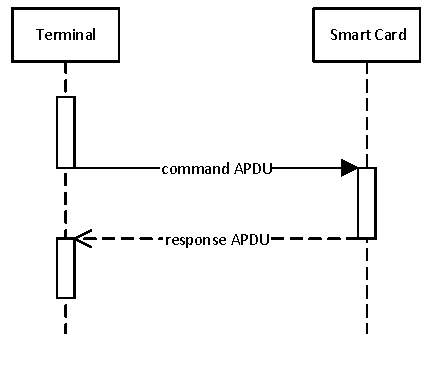
\includegraphics[scale=1, trim=0cm 0cm 0cm 0cm]{figures/apdu}
  \caption{Communication between a terminal and a \jc via command and response APDUs. Figure from~\cite[p. 4]{javasec}.}
  \label{fig:apdu}
\end{figure}
